% --- CONFIGURATION LOCALE DE MISE EN PAGE ---
\begingroup
\onehalfspacing % Interligne 1.5
\setlength{\parskip}{0.8em}
\setlength{\parindent}{0pt}

% =============================================================
% RÉSUMÉ (Français)
% =============================================================
\chapter*{Résumé}
\thispagestyle{noheaderpagenum}
\addcontentsline{toc}{chapter}{Résumé}

\begin{center}
    \vspace{0.5cm}
    \large
    \lipsum[1][1]\\
    \vspace{0.5cm}
    \lipsum[1][1]\\
    \vspace{0.5cm}
    \lipsum[1][1]\\
    \vspace{0.5cm}
    \lipsum[1][1]\\
    \vspace{1.5cm}
    \textbf{Mots-clés :} \lipsum[1][1].
\end{center}
\clearpage

% =============================================================
% ABSTRACT (English)
% =============================================================
\chapter*{Abstract}
\thispagestyle{noheaderpagenum}
\addcontentsline{toc}{chapter}{Abstract}

\begin{center}
    \vspace{0.5cm}
    \large
    \lipsum[1][1]\\
    \vspace{0.5cm}
    \lipsum[1][1]\\
    \vspace{0.5cm}
    \lipsum[1][1]\\
    \vspace{0.5cm}
    \lipsum[1][1]\\
    \vspace{1.5cm}
    \textbf{keywords :} \lipsum[1][1].
\end{center}
\clearpage
\endgroup
% --- FIN DE LA CONFIGURATION LOCALE ---

% =============================================================
% ABSTRACT (ARABIC) - INCLUSION DU PDF
% =============================================================
\clearpage
\phantomsection 

% Image dans la Table des Matières (TOC)
\addcontentsline{toc}{chapter}{\texorpdfstring{\protect\raisebox{-0.2em}{\protect
\includegraphics[height=1.2em]{docs/mulakhas.png}}}{Résumé en arabe}}

% Inclusion de l'abstract arabe généré séparément
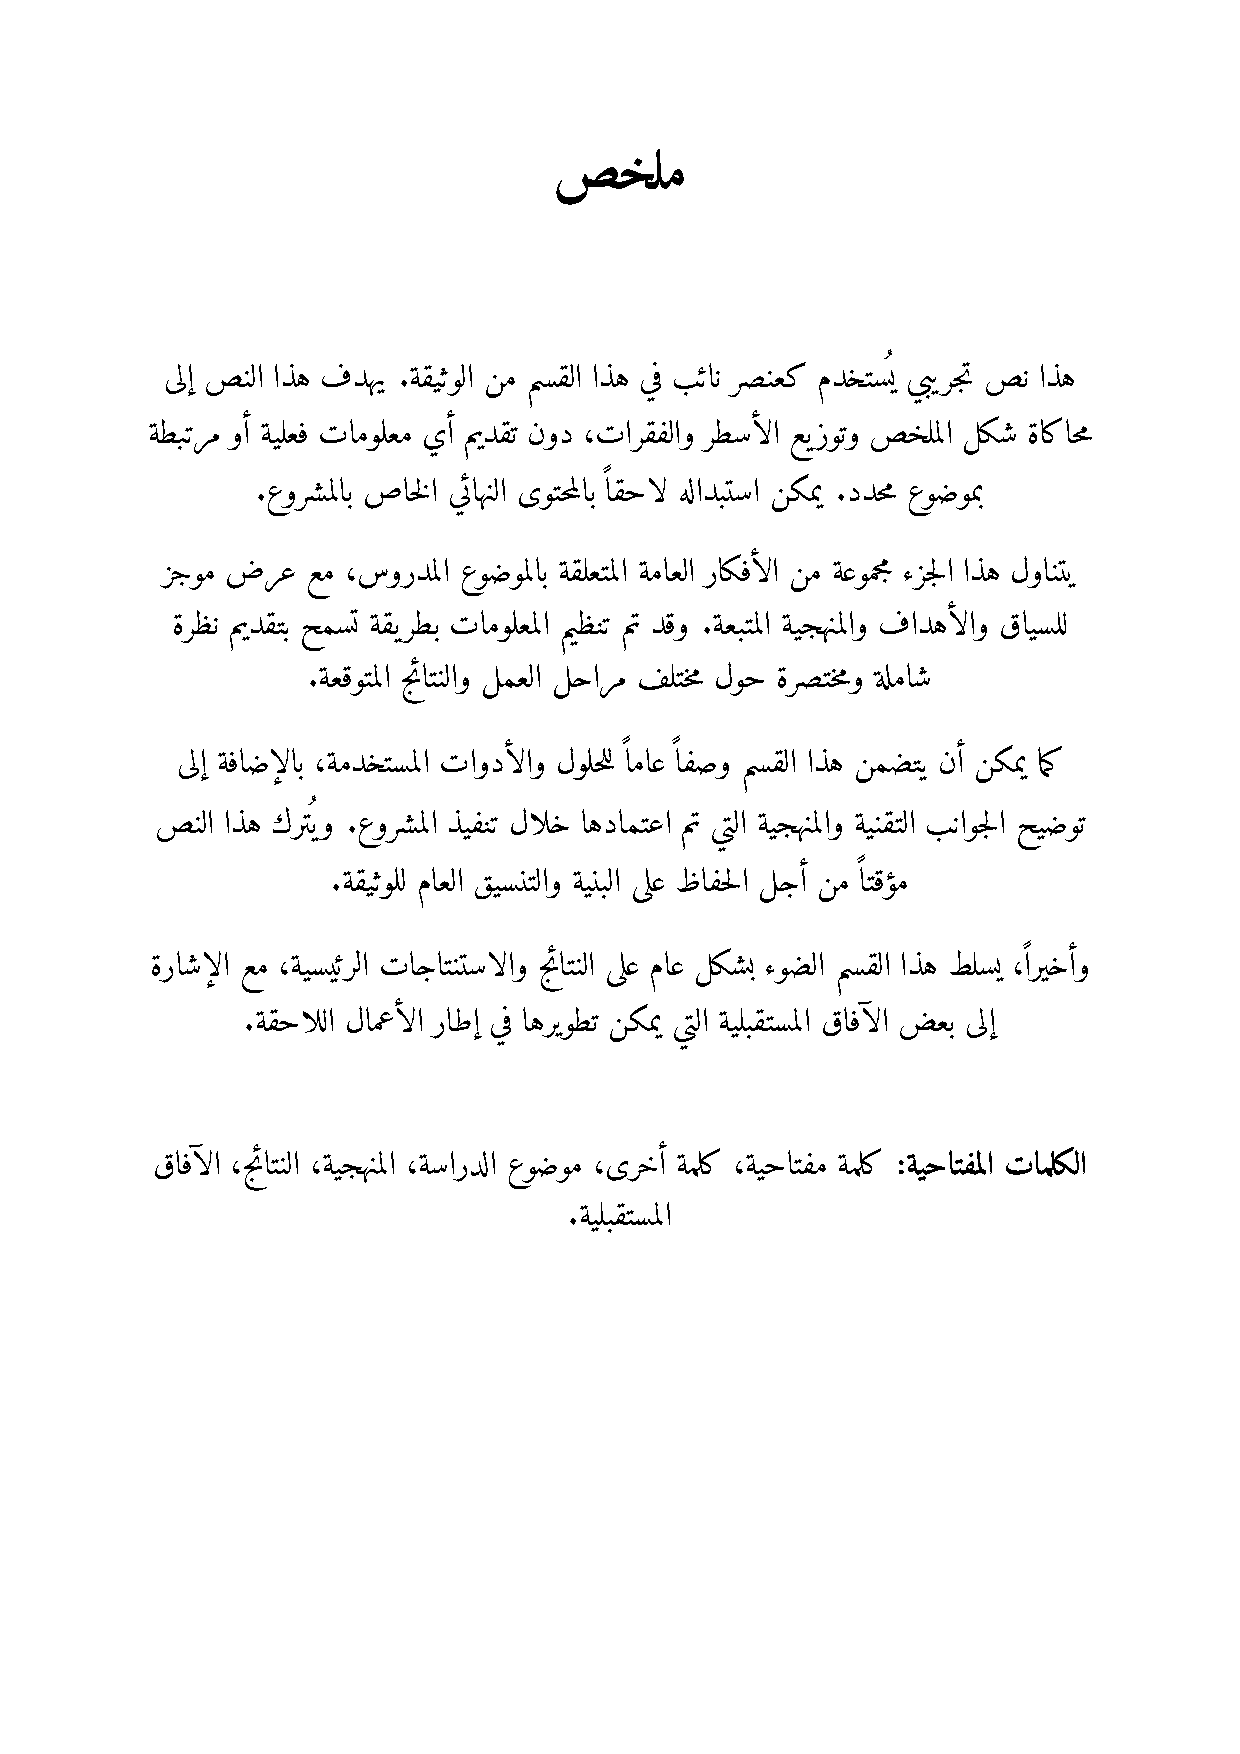
\includepdf[pages=1, pagecommand={\thispagestyle{noheaderpagenum}}]{arabic abstract page/abstract_arabic.pdf}
\clearpage